\begin{figure}[H]
\centering
\shorthandoff{<>}
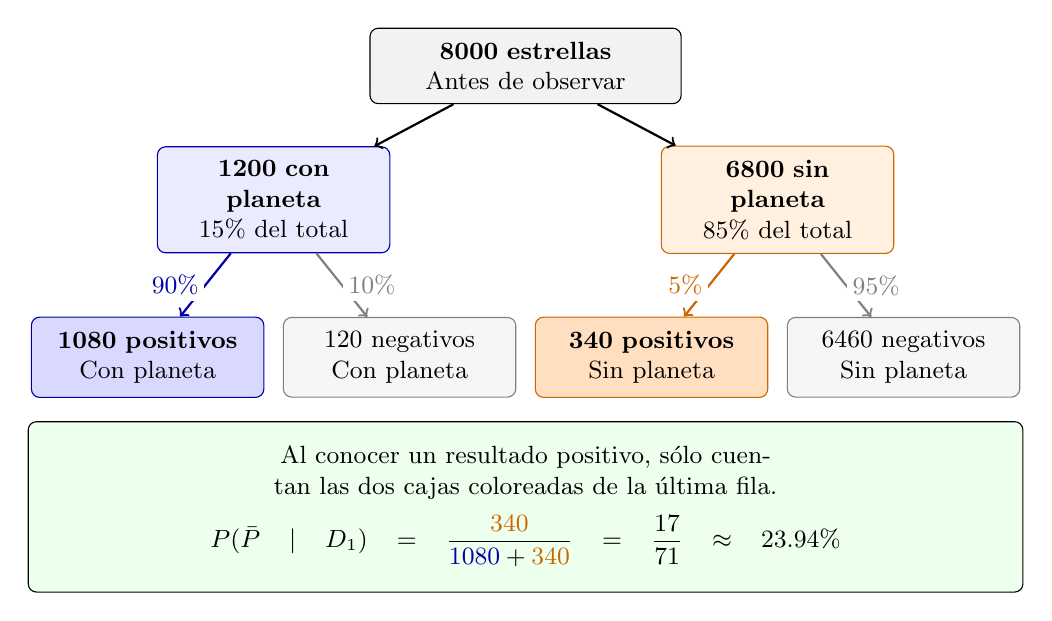
\begin{tikzpicture}[
  font=\small,
  groupbox/.style={draw,rounded corners=3pt,align=center,minimum height=0.9cm,text width=2.6cm,inner sep=5pt},
  connection/.style={->,thick}
]
  \node[groupbox,fill=gray!10,text width=3.6cm] (total) at (0,0)
    {\textbf{8000 estrellas}\\Antes de observar};
  \node[groupbox,draw=blue!65!black,fill=blue!8] (planet) at (-3.2,-1.7)
    {\textbf{1200 con planeta}\\$15\%$ del total};
  \node[groupbox,draw=orange!80!black,fill=orange!12] (noplanet) at (3.2,-1.7)
    {\textbf{6800 sin planeta}\\$85\%$ del total};
  \draw[connection] (total) -- (planet);
  \draw[connection] (total) -- (noplanet);

  \node[groupbox,draw=blue!65!black,fill=blue!15] (truepositive) at (-4.8,-3.7)
    {\textbf{1080 positivos}\\Con planeta};
  \node[groupbox,draw=gray,fill=gray!7] (falsenegative) at (-1.6,-3.7)
    {120 negativos\\Con planeta};
  \node[groupbox,draw=orange!80!black,fill=orange!25] (falsepositive) at (1.6,-3.7)
    {\textbf{340 positivos}\\Sin planeta};
  \node[groupbox,draw=gray,fill=gray!7] (truenegative) at (4.8,-3.7)
    {6460 negativos\\Sin planeta};
  \draw[connection,blue!65!black] (planet) -- (truepositive)
    node[midway,left,fill=white,inner sep=2pt] {$90\%$};
  \draw[connection,gray] (planet) -- (falsenegative)
    node[midway,right,fill=white,inner sep=2pt] {$10\%$};
  \draw[connection,orange!80!black] (noplanet) -- (falsepositive)
    node[midway,left,fill=white,inner sep=2pt] {$5\%$};
  \draw[connection,gray] (noplanet) -- (truenegative)
    node[midway,right,fill=white,inner sep=2pt] {$95\%$};

  \node[draw,rounded corners=3pt,fill=green!7,align=center,text width=12cm,inner sep=9pt] at (0,-5.6)
    {Al conocer un resultado positivo, sólo cuentan las dos cajas coloreadas de la última fila.\\[5pt]
    $\displaystyle P(\bar P\mid D_1)
      =\frac{\textcolor{orange!80!black}{340}}
      {\textcolor{blue!65!black}{1080}+\textcolor{orange!80!black}{340}}
      =\frac{17}{71}\approx23.94\%$};
\end{tikzpicture}
\shorthandon{<>}
\caption{Bayes mediante frecuencias esperadas en una población ilustrativa de 8000 estrellas, no mediante datos observados. El $5\%$ se aplica a las 6800 estrellas sin planeta; el $23.94\%$ se calcula entre los 1420 resultados positivos. Son probabilidades con distintos denominadores.}
\label{fig:bayes-frecuencias}
\end{figure}